\subsection*{\hypertarget{world}{Worldbuilding}}
\addcontentsline{toc}{subsection}{Worldbuilding}%
"World very simple place. World only have two things: things you can eat and things you no can eat."\\
\indent -- Quina

\begin{center} 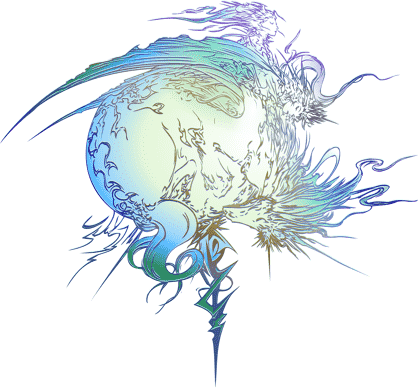
\includegraphics[width=1\columnwidth]{./art/images/ff13.png} \end{center}
\noindent
Creating a world is one of the most difficult, but also most rewarding parts of being a GM.
The players become part of your world, where they interact with the environment and change it through their actions and decisions. 
Therefore, the world should catch their curiosity by offering interesting content and allowing meaningful choices.
This subsection gives some suggestions on how to create an interesting game world.

\subsubsection*{Central Conflict}
Most adventures revolve around a central conflict, which the party aims to solve as the goal of their adventure.
Traditionally, this conflict involves multiple forces with opposing interests and the adventurers can be part of either of these sides.
Accordingly, there is also an opposing side, a common enemy or antagonist that acts against the party.
As the GM, you take the role of characters on different sides of this conflict, so you need to consider their different perspectives. 

\subsubsection*{Map}
A good way to start building an adventure is to establish what the world looks like on a map. 
Begin by creating its natural layout including landmass, water, forests, mountains and deserts. 
Afterwards, place and mark locations that could be interesting for players to visit, like cities, dungeons or ruins.
Then add more detail only to the places that the players will likely visit in the beginning, you can do the rest later on.
You may provide the players with this map at some point in the game to make them aware of these locations you have created.

\pagebreak

\subsubsection*{Non-Player Characters}
After creating some detailed locations, think about who might live in these places.
These non-player characters are roleplayed by you when interacting with the party.
They live their own lives, independent of the players and have their own personalities, goals, abilities and outlooks on life. 
Accordingly, they often have knowledge about the world that the players do not.
They can be allied, neutral or enemies of the party depending on the circumstances.
For creating detailed non-player characters, use the \hyperlink{char}{Character Creation Guide}, but usually it is sufficient to write down some notes on them.

\subsubsection*{Magic}
There are two fantasy elements that are deeply ingrained into the game system: magic and monsters.
For magic it is important to establish its sources and what role it plays in your world.
In Final Fantasy, crystals are often portrayed as powerful sources of magic and are thus at the center of many conflicts.
Often there are also magical beings called \hyperlink{summons}{Espers}, who represent the different forces of nature and are connected to the crystals.
Monsters are usually connected to the magic sources in some way as well, so they are able to use magic. 

\subsubsection*{Technology}
The progression of technology is another important aspect that significantly shapes your game world.
Different technologies, such as machines and weapons, can complement the magical forces in the world, but may also stand in conflict against them.
Thus, the societies of your world may prefer and rely on magic and technology to varying degrees in their daily lives.
During their adventure, the party can make use of available technologies and might even contribute to the current state of art.

\vspace{0.8cm}

\example{Worldbuilding}
{
	The world we create consists two parts: Pulse and Cocoon.
	Pulse is a huge uncharted planet with a vast nature that is home to various monsters.
	In contrast, Cocoon is a small planet that floats above Pulse and is inhabited by an advanced human society.
	The Cocoon citizen depend on the god-like beings for necessities such as food and electricity.
	These powerful beings are called fal'Cie and can directly or indirectly assert control over humans.
	The fal'Cie of Cocoon stand in conflict against the fal'Cie of Pulse and accordingly humans are conditioned to be hostile towards Pulse.		
	Our adventure starts on Cocoon, where an ancient Pulse fal'Cie has been discovered some days ago.
	In a radical answer, the Cocoon government orders the deportation of all humans that have been near the Pulse fal'Cie.
	Small rebellion groups form among the citizen to fight back against this so-called "Purge".
}

\pagebreak






